\documentclass[11pt]{scrartcl}
\usepackage{graphicx}
\title{\textbf{HTML5 key frame based videoplayer}}
\author{\emph{Peter Spiess-Knafl, Armin Trattnig}}
\begin{document}
\date{}
\maketitle

\section{Motivation}
We decided to choose this project, because it was the most interesting one for both of us. And we also thought that a good videobrowser could be useful in everyday life. Also none of us had good practice in HTML5/JavaScript programming.

\begin{center}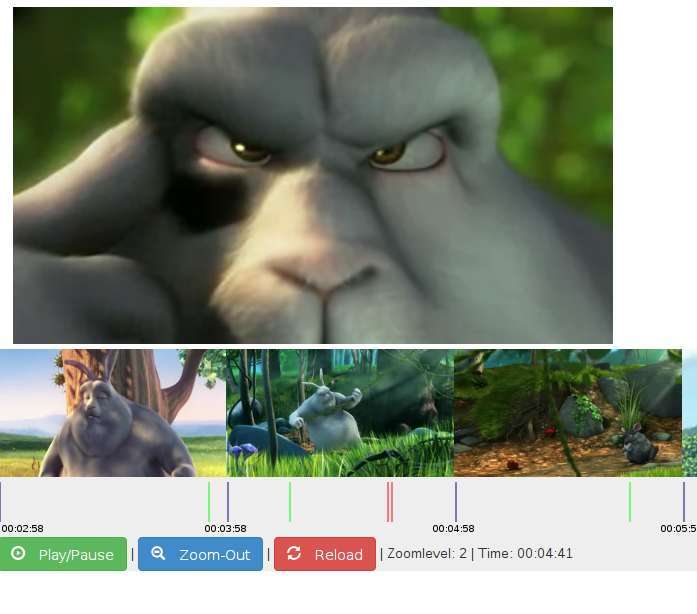
\includegraphics[scale=0.5]{screenshot}\end{center}

\section{Implementation}

\subsection{Userinterface}
We used Bootstrap\footnote{http://getbootstrap.com} for a nice looking userinterface, because we are no experts at all in webdesign.

\subsection{Architecture}
We split the source code in two main fragments:
\begin{itemize}
\item index.html: contains all visible HTML elements (player, timeline, keyframes, buttons).
\item videoplayer.js: contains the actual implementation of the videoplayer.
\end{itemize}

\subsection{Important functions}
There are three main functions which are important for the videoplayer:
\begin{itemize}
\item \emph{initThings()}: This function binds all variables to the HTML tags by using jQuery\footnote{http://jquery.com}
\item \emph{drawThumbs()}: Extracts random keyframes according to the zoomlevel.
\item \emph{newTimeline()}: Draws everything visible on the timeline (timestamps, key frame references, current playbacktime).
\end{itemize}

\section{Problems}

We ran into several problems during the programming phase: 

\subsection{Frame extraction}
This was the first problem we ran into. How can we extract Frames from future timestamps, while the player is playing the video at the current playback time? 

The HTML5 \emph{video tag} does not have native support for that. So we decided to clone the existing video tag and use this one for frame extraction. 
\\
With the \emph{seeked event}, we were able to extract future frames or even frames at a random time in the video, without disturbing the current playback.

\subsection{The timeline}
The timeline was a very challenging part, because we got no support by any existing HTML5 objects, beside a plain canvas field. So we had to render everything that is visible on the timeline manually:

\begin{itemize}
	\item Current time resolution (blue lines)
	\item Current playback spot (red line)
	\item Reference to key frames (green lines)
	\item Timestamps according to current zoomlevel/playbacktime
\end{itemize}

Especially the zoomfactor required a lot of thinking, to calculate the right X-Pixel-Offset on the canvas and also the corresponding timesets (in HH:MM:SS).

\subsection{Zooming}
At first we choose a Zoomfactor of 1 / N (Number of keyframes) on each zooming-step. But especially for our testing video (which was about 10 minutes long). This approach was not very satisfying, because after two times zoooming, you could see only familiar frames. 

So we decided to choose a constant Zoomingfactor of 2. This gave us far better results in the random key-frame extraction and is still sufficient for longer videos.

\section{Conclusio}

We have learned a lot about HTML5/Javascript coding, and it was quite fun. A very nice effect was, that we actually build something that we can make use of in everyday life. It is a powerful tool.

\end{document}
